\section{Vergleich der \qlearning und \sarsa Agenten}

Die trainierten Agenten beider Algorithmen konnten erfolgreich \acl{TTT} durch \splay lernen und Spielstärken erreichen, die über dem implementierten Minimax-Algorithmus liegen. 
\cref{tab:playingAbility_compareAlgorithms_normal} vergleicht die Spielstärke von \bothAlgs, die mit klassischem \splay trainiert wurden. 
Für jede untersuchte Lernrate war die Spielstärke der \qlearning Agenten größer als die von \sarsa. 
\cref{tab:playingAbility_compareAlgorithms_alternate} vergleicht die Spielstärke, die bei alternierendem \splay erreicht werden kann. 
Im Gegensatz zum klassischen \splay erreichen die \sarsa Agenten eine höhere Spielstärke. 
Die \qlearning Agenten verschlechtern sich deutlich bei alternierendem \splay und sind schlechter als der Minimax-Algorithmus. 
Für beide Algorithmen werden mit dem klassischen \splay bessere Ergebnisse erzielt. 
Der jeweils stärkste Agent konnte für $\alpha=0,1$ mit klassischem \splay erzeugt werden. 
Für \qlearning beträgt die durchschnittliche Spielstärke 8.002,72 und für \sarsa 7.905,72. 
Für 150.000 Trainingsepisoden weist \sarsa noch eine leichte Schwäche vor und verliert als Symbol O knapp 1\% seiner Spiele.


Die Verwendung von Afterstates in Form der \wtable verbesserte bei beiden Agenten die Konvergenz.
\cref{fig:convergence_compare_algorithm} vergleicht den Verlauf der Rate optimaler Aktionen während dem Training. Für Symbol X und Symbol O konvergiert der \qlearning Agent schneller und erreicht eine höhere Rate. 
Zudem verbesserte sich die durchschnittliche Spielstärke beider Agenten, wie \cref{tab:playingAbility_compareAlgorithms_experience} zeigt. 
Der \qlearning Agent verbesserte seine Spielstärke um 33,96 auf 8.036,68. 
Die Schwäche von \sarsa wird behoben, sodass dieser als Symbol O keine Spiele mehr verliert.
Die Spielstärke verbessert sich dadurch um 21,96 auf 7.927,68.
Wie jedoch in den jeweiligen Abschnitten angemerkt, ist diese Verbesserung in Relation zur Standardabweichung klein und es liegt nur eine Stichprobenanzahl von $N=5$ vor.

\begin{table}
\centering
\caption[Spielstärke beider Algorithmen unterschiedliche Lernraten, klassisches \splay]{Spielst"arke beider Algorithmen für unterschiedliche Lernraten nach Training mit klassischem \splay}
\label{tab:playingAbility_compareAlgorithms_normal}

\begin{tabular}{lrrr}
\toprule
Lernrate $\alpha$               & Spielst"arke Q-Learning           & Spielst"arke Sarsa                & Differenz QL - Sarsa \\ \midrule
Konstant 0,1                    & 8.002,72 $\pm$ \phantom{0}30,03   & 7.905,72 $\pm$ \phantom{0}75,69   & 97,00 \\
Konstant 0,2                    & 7.801,36 $\pm$ 131,22             & 7.787,94 $\pm$ 105,20             & 13,42 \\
Abnehmend 1 $\rightarrow$ 0,1   & 7.894,92 $\pm$ 132,52             & 7.754,66 $\pm$ 197,59             & 140,26 \\ \bottomrule

\end{tabular}
\end{table}
\begin{table}
\centering
\caption[Spielstärke beider Algorithmen unterschiedliche Lernraten, alternierendes \splay]{Spielst"arke beider Algorithmen für unterschiedliche Lernraten nach Training mit alternierendem \splay}
\label{tab:playingAbility_compareAlgorithms_alternate}

\begin{tabular}{lrrr}
\toprule
Lernrate $\alpha$               & Spielst"arke Q-Learning           & Spielst"arke Sarsa                & Differenz QL - Sarsa \\ \midrule
Konstant 0,1                    & 6.465,66 $\pm$ 481,99             & 6.495,50 $\pm$ 826,74             & \textcolor{red}{-29,84} \\
Konstant 0,2                    & 6.904,92 $\pm$ 399,15             & 7.018,94 $\pm$ 299,04             & \textcolor{red}{-114,02} \\
Abnehmend 1 $\rightarrow$ 0,1   & 6.110,56 $\pm$ 224,66             & 7.625,94 $\pm$ \phantom{0}65,10   & \textcolor{red}{-1.515,38} \\ \bottomrule
\end{tabular}
\end{table}
\begin{table}
\centering
\caption[Spielstärke beider Algorithmen mit \qtable und \wtable, klassisches \splay]{Spielstärke beider Algorithmen mit \qtable und \wtable, klassisches \splay}
\label{tab:playingAbility_compareAlgorithms_experience}

\begin{tabular}{lrrr}
\toprule
Algorithmus                & Spielst"arke Q-Tabelle     & Spielst"arke W-Tabelle              & Q-Tabelle - W-Tabelle \\ \midrule
Q-Learning $\alpha=0,1$    & 8.002,72 $\pm$ 75,69      & 8.036,68 $\pm$ \phantom{0}9,13    & 33,96 \\
Sarsa $\alpha=0,1$         & 7.905,72 $\pm$ 30,03      & 7.927,68 $\pm$ 43,79               & 21,96 \\ \bottomrule
\end{tabular}
\end{table}

\begin{figure}
\centering
\begin{subfigure}[b]{0.75\textwidth}
    \centering
   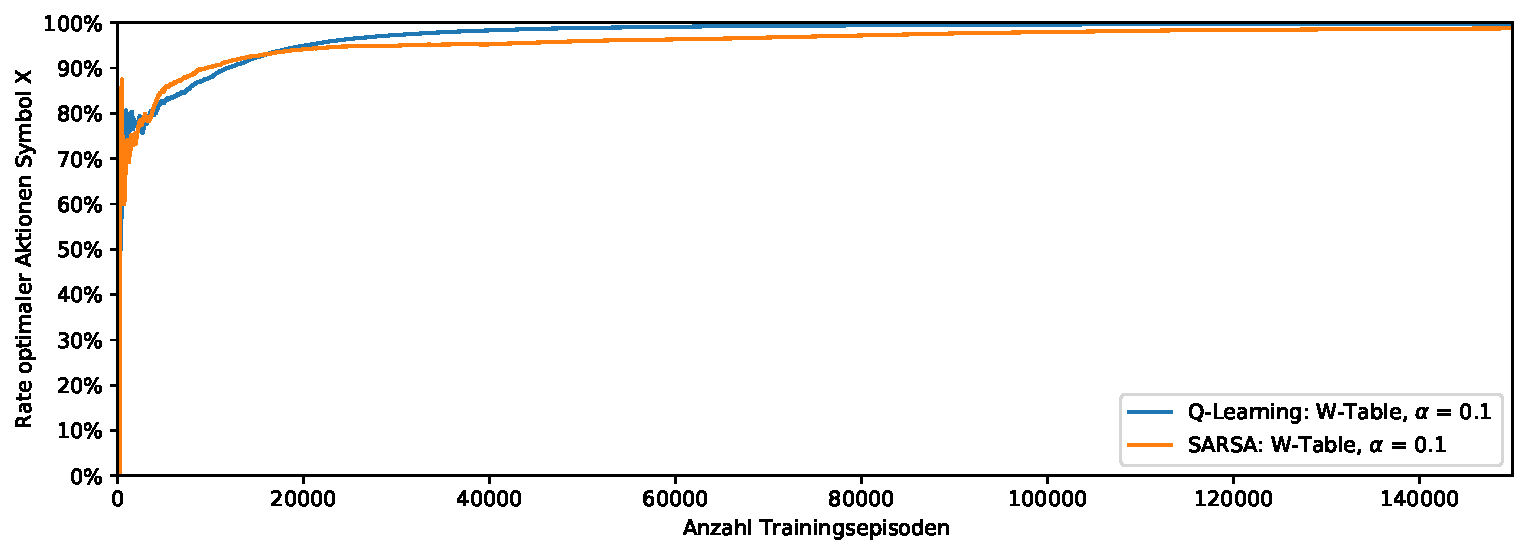
\includegraphics[width=1\linewidth]{convergence/convergence_compare_algorithm_X.pdf}
   \caption{Symbol X}
   \label{fig:convergence_compare_algorithm_X} 
\end{subfigure}

\begin{subfigure}[b]{0.75\textwidth}
    \centering
   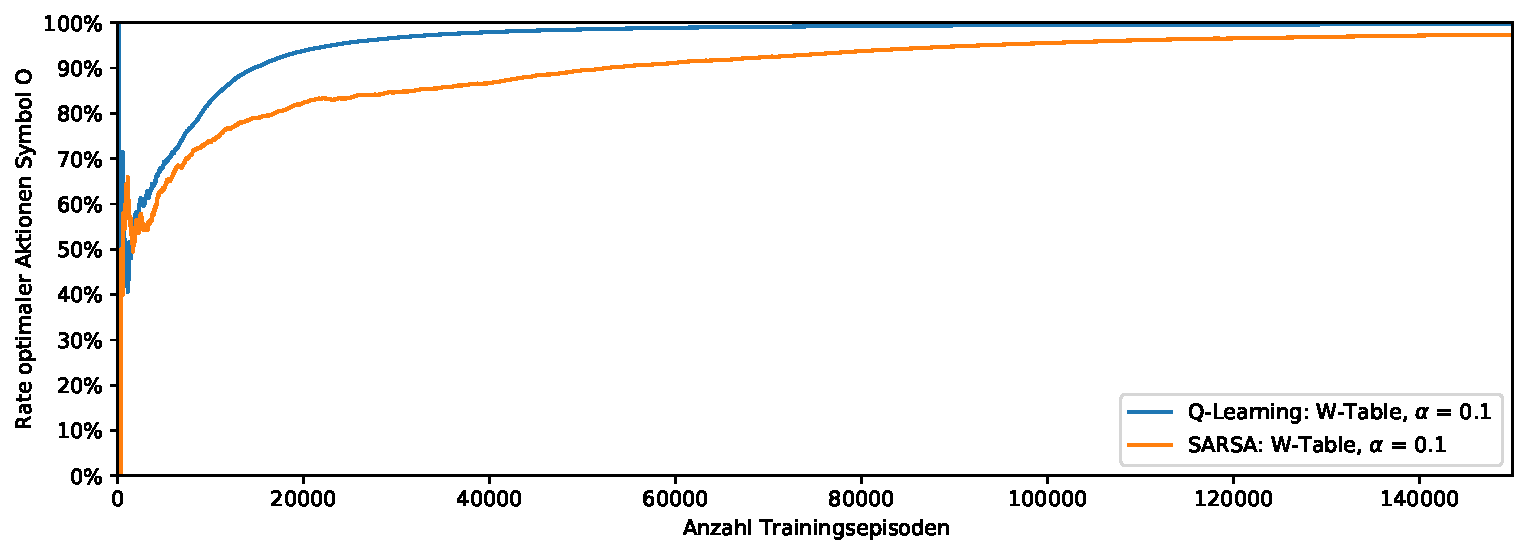
\includegraphics[width=1\linewidth]{convergence/convergence_compare_algorithm_O.pdf}
   \caption{Symbol O}
   \label{fig:convergence_compare_algorithm_O}
\end{subfigure}


\caption[Rate optimaler Aktionen bester \qlearning und \sarsa Agent, \wtable, klassisches \splay]{Rate optimaler Aktionen des besten \qlearning und \sarsa Agenten während dem Training mit \wtable und klassischem \splay (a) Symbol X (b) Symbol O}
\label{fig:convergence_compare_algorithm}
\end{figure}